\documentclass[12pt]{jarticle}
\usepackage[dvipdfmx]{graphicx}
\usepackage{url}
\usepackage{listings,jlisting}
\usepackage{ascmac}
\usepackage{amsmath,amssymb}

%ここからソースコードの表示に関する設定
\lstset{
  basicstyle={\ttfamily},
  identifierstyle={\small},
  commentstyle={\smallitshape},
  keywordstyle={\small\bfseries},
  ndkeywordstyle={\small},
  stringstyle={\small\ttfamily},
  frame={tb},
  breaklines=true,
  columns=[l]{fullflexible},
  numbers=left,
  xrightmargin=0zw,
  xleftmargin=3zw,
  numberstyle={\scriptsize},
  stepnumber=1,
  numbersep=1zw,
  lineskip=-0.5ex
}
%ここまでソースコードの表示に関する設定

\title{知能プログラミング演習II 課題4}
\author{グループ8\\
  29114003 青山周平\\
}
\date{2019年11月11日}

\begin{document}
\maketitle

\paragraph{提出物} rep4
\paragraph{グループ} グループ8
\paragraph{メンバー}
\begin{tabular}{|c|c|c|}
  \hline
  学生番号&氏名&貢献度比率\\
  \hline\hline
  29114003&青山周平&20\\
  \hline
  29114060&後藤拓也&20\\
  \hline
  29114116&増田大輝&20\\
  \hline
  29114142&湯浅範子&20\\
  \hline
  29119016&小中祐希&20\\
  \hline
\end{tabular}



\section{課題の説明}
\begin{description}
\item[必須課題4-1] まず,教科書3.2.1の「前向き推論」のプログラムと教科書3.2.2の「後向き推論」のプログラムとの動作確認をし,前向き推論と後ろ向き推論の違いを説明せよ.また,実行例を示してルールが選択される過程を説明せよ.説明の際には,LibreOfficeのDraw(コマンド soffice --draw)などのドロー系ツールを使ってp.106 図3.11やp.118 図3.12のような図として示すことが望ましい.
\item[必須課題4-2] CarShop.data , AnimalWorld.data 等のデータファイルを実際的な応用事例(自分達の興味分野で良い)に書き換えて,前向き推論,および後ろ向き推論に基づく質問応答システムを作成せよ.どのような応用事例を扱うかは,メンバーで話し合って決めること.
なお,ユーザの質問は英語や日本語のような自然言語が望ましいが,難しければ変数を含むパターン等でも可とする.
\item[必須課題4-3] 上記4-2で実装した質問応答システムのGUIを作成せよ.
質問に答える際の推論過程を可視化できることが望ましい.
\item[発展課題4-4] 上記4-3で実装したGUIを発展させ,質問応答だけでなく,ルールの編集(追加,削除,変更)などについてもGUIで行えるようにせよ.
\end{description}

\section{必須課題4-3}
\begin{screen}
上記4-2で実装した質問応答システムのGUIを作成せよ.
質問に答える際の推論過程を可視化できることが望ましい.
\end{screen}
私の担当箇所は,必須課題4-3におけるGUIの,Swingによる実装である.

\subsection{手法}
まず,前向き推論のためのGUIを実装するにあたり,以下のような方針を立てた.
\begin{enumerate}
\item 推論のルール・推論結果を受け取る.
\item 推論過程を可視化するためのパネルを作る.
\end{enumerate}

1.に関して,MVPアーキテクチャを導入し,Presenterを他の班員に作ってもらい,それを介してデータを受け取ることで,ModelであるRuleBaseSystem.javaとの独立性の高いGUIを設計できるような仕様とした.

2.に関して,表示パーツの部品化や配置を工夫することで,ユーザにとって統一的な表示がなされるように心がけた. \\

次に,後向き推論のためのGUIを実装するにあたり,以下のような方針を立てた.
\begin{enumerate}
\item 前向き推論のクラスを部品化して活用する.
\end{enumerate}

1.に関して,前向き推論で制作したFwdChainTableクラスをChainTableクラスで抽象化することで,プログラム全体の多層化を高めた.また,これにより前向き推論と後向き推論の互換性を高めることによって,プログラム全体がまとまりを持つような仕様とした.

\subsection{実装}
双方の推論に共通するプログラムChainGUI.java,StepPanel.javaには以下のクラスが含まれる.
\begin{description}
\item[ChainGUI] メニューパネルといった,FwdChainGUI,BwdChainGUIの共通部分を管理するための親クラス.
\item[ChainTable] FwdChainTable,BwdChainTableを管理するための抽象クラス.
\item[StepPanel] 導出の各ステップを表示するためのクラス.
\item[EdgePanel] 導出のステップ間の繋がりを管理するためのクラス.
\end{description}

前向き推論のGUIに関するプログラムBwdChainGUI.javaには以下のクラスが含まれる.
\begin{description}
\item[FwdChainGUI] メソッドmainを実装した,フレームを実装するためのクラス.
\item[FwdChainTable] 前向き推論のアサーション・ルール・過程などを管理・表示するパネルを実装するためのクラス.
\end{description}

後向き推論のGUIに関するプログラムBwdChainGUI.javaには以下のクラスが含まれる.
\begin{description}
\item[BwdChainGUI] メソッドmainを実装した,フレームを実装するためのクラス.
\item[BwdChainTable] 後向き推論のアサーション・ルール・過程などを管理・表示するパネルを実装するためのクラス.
\end{description}

\subsubsection{推論のルール・推論結果を受け取る}
推論を行う上で,RuleBaseSystem.javaとデータのやりとりをして前提条件の引き渡しと結果の受け取りをできるようにする必要があった.そこで,他の班員にGUIとRuleBaseSystem.javaとの仲介を行うプログラムPresenter.javaを制作してもらい,FwdChainGUIでは,Presenter型のフィールドpresを用いて以下のようにデータの受け渡しをコンストラクタに組み込んだ.

\begin{lstlisting}[caption=FwdChainTableクラスのコンストラクタ, label=fwdcons]
    FwdChainTable(String fileName) {
        super(fileName);
        view = new View();
        pres = new Presenter(view);
        pres.start(new ArrayList<String>(), fileName);
        ...
    }
\end{lstlisting}

データの受取についても同様に行った.例として質疑応答の結果を受け取るプログラムをソースコード
\ref{schstep}に示す.

\begin{lstlisting}[caption=FwdChainTableクラスのメソッドschStep, label=schstep]
    void schStep(ArrayList<String> astList, ArrayList<String> schAst) {
        ...
        pres.restart(astList);
        ArrayList<StepResult> stepList = pres.stepResult();  // 全ルートの受け取り
        paintPnls(stepList);

        if (schAst.get(0).equals("")) {
            System.out.println("WARNING: 検索文の格納に失敗");
        } else {
            ArrayList<ArrayList<SearchStep>> resList = pres.searchAssertion(schAst);  // 質疑応答結果の受け取り
            answerPnls(resList.get(0));
        }
    }
\end{lstlisting}

これらのデータの受取の実装は,Presenterの制作と同時並行して行ったため,Presenterに渡す変数の個数や型,Presenterから受け取る形などに実装を窮したが,密に班員とコニュニケーションを取ることにより,細かい仕様をすり合わせて実装まですることができた.

\subsubsection{推論過程を可視化するためのパネルを作る.}
推論における各ステップについてStepPanelインスタンスを作り,StepPanel間の繋がりを表示するためにEdgePanelを作ることで,推論の可視化を行った.

StepPanelのコンストラクタは,以下に示すように2種類のコンストラクタを持つ.

\begin{lstlisting}[caption=StepPanelクラスのコンストラクタ2種, label=stepconst]
    StepPanel(Assertion ast) {
        setLayout(new BoxLayout(this, BoxLayout.PAGE_AXIS));
        setBackground(Color.ORANGE);
        setBorder(new BevelBorder(BevelBorder.RAISED));
        setSize(200, 30);
        setLocation(10, 10);

        alabel = new JLabel(ast.getName());
        add(alabel);
    }

    StepPanel(StepResult step) {
        setLayout(new BoxLayout(this, BoxLayout.PAGE_AXIS));
        setBackground(Color.ORANGE);
        setBorder(new BevelBorder(BevelBorder.RAISED));
        setSize(200, 150);
        setLocation(10, 10);

        Rule apply = step.getApply();
        if (apply != null) {
            JPanel rpanel = new RulePanel(apply);
            add(rpanel);
        }

        JLabel alabel = new JLabel(" => " + step.getSuccess().getName());
        add(alabel);
    }
\end{lstlisting}

これらはインスタンス生成時に渡される引数の型によって挙動が異なることを意味する.すなわち,1つ目のインスタンスでワーキングメモリ用のStepPanelと,ルールとそのルールから得られた結果である推論過程を,同じStepPanelクラスで同一的に管理できるような仕様としたことが分かる.

これにより,EdgePanelの管理も容易になる.StepPanelの位置関係のみから,それらの繋がりを表示するためのStepPanelのコンストラクタと描写に関するメソッドを以下に示す.

\begin{lstlisting}[caption=StepPanelクラスのコンストラクタとpaintComponent,paintArrowsメソッド, label=edge]
    EdgePanel(StepPanel topPnl, StepPanel btmPnl) {
        this.topPnl = topPnl;
        this.btmPnl = btmPnl;
        grace = 10;
        pass = false;
        topPoint = new Point(topPnl.getX() + (topPnl.getWidth() / 2), topPnl.getY() + topPnl.getHeight());
        btmPoint = new Point(btmPnl.getX() + (btmPnl.getWidth() / 2), btmPnl.getY());

        int lpX = getLeft();
        int lpY = getTop();
        int lpWidth = getRight() - lpX;
        int lpHeight = getBtm() - lpY;
        setBounds(lpX, lpY, lpWidth, lpHeight);

        setOpaque(false); // パネルの透過
    }

    @Override
    public void paintComponent(Graphics g) {
        super.paintComponent(g);
        Graphics2D g2d = (Graphics2D) g;
        paintArrows(g2d);
    }

    void paintArrows(Graphics2D g) {
        int fromX = topPoint.x;
        int fromY = topPoint.y;
        int toX = btmPoint.x;
        int toY = btmPoint.y;

        // 相対座標の考慮
        int relX = getLeft();
        int relY = getTop();

        if (pass) {
            g.setColor(Color.RED);
        } else {
            g.setColor(Color.BLUE);
        }
        BasicStroke stroke = new BasicStroke(2.0f);
        g.setStroke(stroke);
        g.drawLine(fromX - relX, fromY - relY, toX - relX, toY - relY);
    }
\end{lstlisting}

描写に関して,Graphics2Dクラスを活用することで,より太く見やすい線の描写が実現されている.

次に,各StepPanelをどのような位置関係で配置するかをFwdChainGUI側で設定する必要があった.そこで,そのためのメソッドpaintPnls,traceParを以下のように作った.

\begin{lstlisting}[caption=FwdChainGUIクラスのメソッドpaintPnls,tracePar, label=steplocation]
    void paintPnls(ArrayList<StepResult> srList) {
        stepMap.clear();
        edgeMap.clear();
        locMap.clear();

        for (StepResult sr : srList) {
            tracePar(sr);
        }
    }

    void tracePar(StepResult sr) {
        if (sr.getAddSR() != null) {
            for (StepResult from : sr.getAddSR()) {
                tracePar(from); // 再帰
            }
            StepPanel sp = stepMap.get(sr);
            if (sp == null) {
                sp = new StepPanel(sr);
                stepMap.put(sr, sp);
                add(sp);

                Integer locY = stepMap.get(sr.getAddSR().get(0)).getY() + next;
                Integer preX = locMap.get(locY);
                Integer locX = 10;
                if (preX != null) {
                    locX = preX + next;
                }
                locMap.put(locY, locX);
                sp.setLocation(locX, locY);
            }

            for (StepResult from : sr.getAddSR()) {
                StepPanel fromPnl = stepMap.get(from);
                EdgePanel ep = new EdgePanel(fromPnl, sp);
                edgeMap.put(sr, ep);
                add(ep);
            }
        } else {
            if (!stepMap.containsKey(sr)) {
                StepPanel sp = new StepPanel(sr.getSuccess()); // ここで作ったり
                stepMap.put(sr, sp);
                add(sp);

                Integer locY = 10;
                Integer preX = locMap.get(locY);
                Integer locX = 10;
                if (preX != null) {
                    locX = preX + next;
                }
                locMap.put(locY, locX);
                sp.setLocation(locX, locY);
            }
        }
    }

\end{lstlisting}

traceParメソッドから分かるように,この処理は再帰的に行われている.すなわち,導出の各ステップを保持するStepResult型の変数がフィールドに持つ,自身のアサーションがどこから生成されたかのリンクを用いて,初期値で渡されるワーキングメモリまで辿られていることが分かる.すなわち,導出の順番と可視化される配置が同じになるように処理がなされている.また,パネル同士が重ならないように,locMapというマップで座標の管理がなされている.

また,stepMapやedgeMapでは,同じ推論過程に関するStepPanelやEdgePanelが重複して生成されないかの管理が行われている.


\subsubsection{前向き推論のクラスを部品化して後向き推論に活用する.}
後述する発展課題4-4でも述べるが,ここでは特にStepPanel.javaの資源活用について述べる.元々は後向きでも前向きでも同一のStepPanel.javaで動作するように設計していたのだが,Presenter側の抽象化が難しかったので,前向き・後向きそれぞれでStepPanel.javaを持つこととした.

しかし,その設計の名残の恩恵もあり,Presenterの型と用いるメソッドの引数や名前を変えるだけで,他はほとんど手を加えずに後向き推論の実装もできた.
\clearpage

\subsection{実行例}
FwdChainGUIを実行したところ,下図のような画面が得られる.

\begin{figure}[!hbt]
  	\begin{center}
  		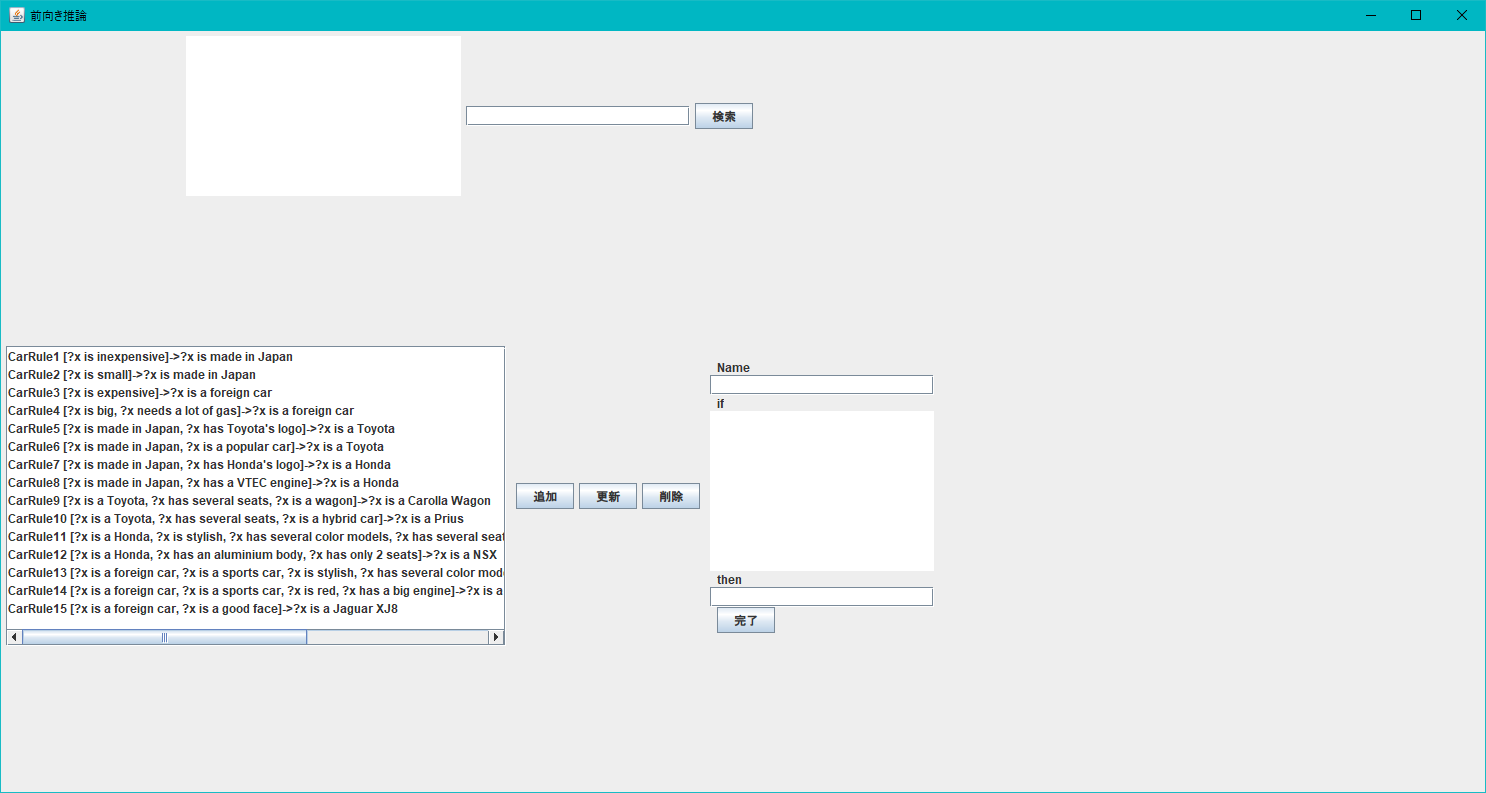
\includegraphics[scale=0.35]{images/gui1.png}
	\end{center}
  	\caption{FwdChainGUI初期状態}
\end{figure}
\clearpage

FwdChainGUIを実行したところ,下図のような画面が得られる.

\begin{figure}[!hbt]
  	\begin{center}
  		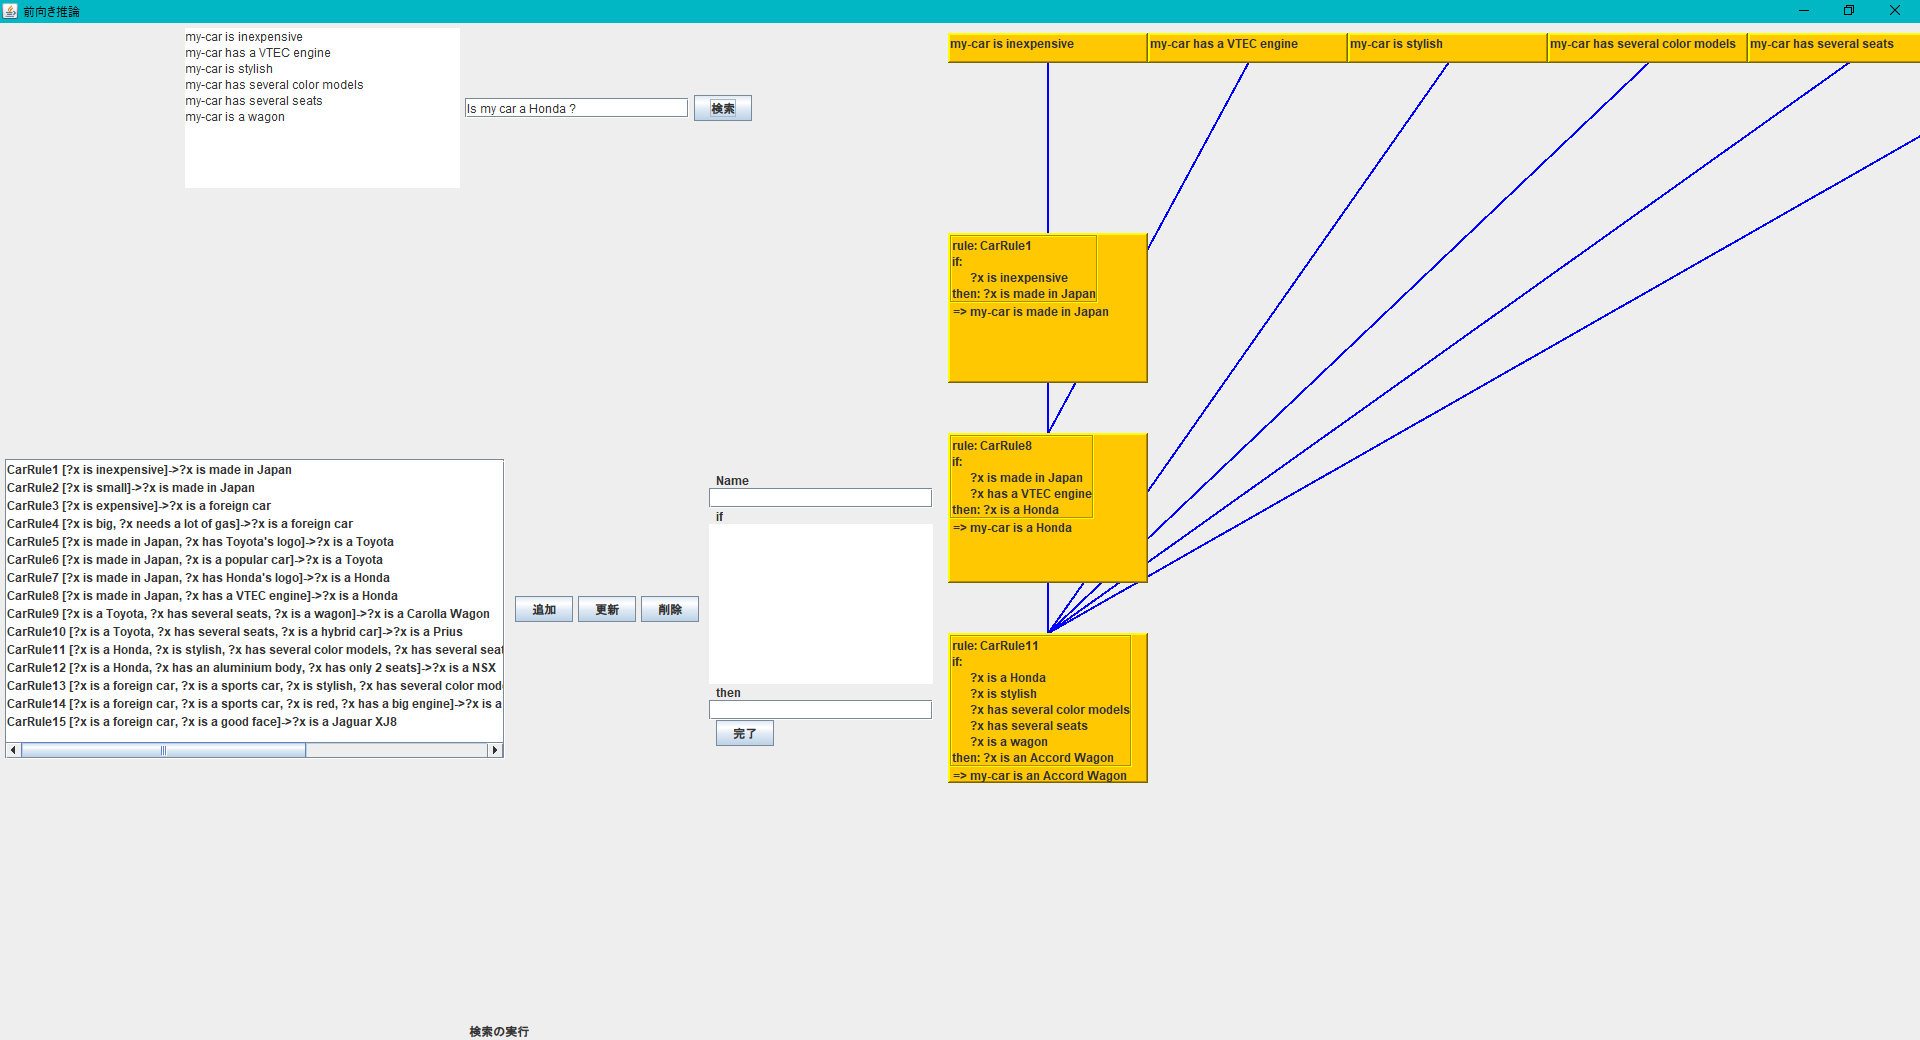
\includegraphics[scale=0.25]{images/gui2.png}
	\end{center}
  	\caption{前向き推論過程を可視化}
\end{figure}
\clearpage

BwdChainGUIを実行したところ,下図のような画面が得られる.

\begin{figure}[!hbt]
  	\begin{center}
  		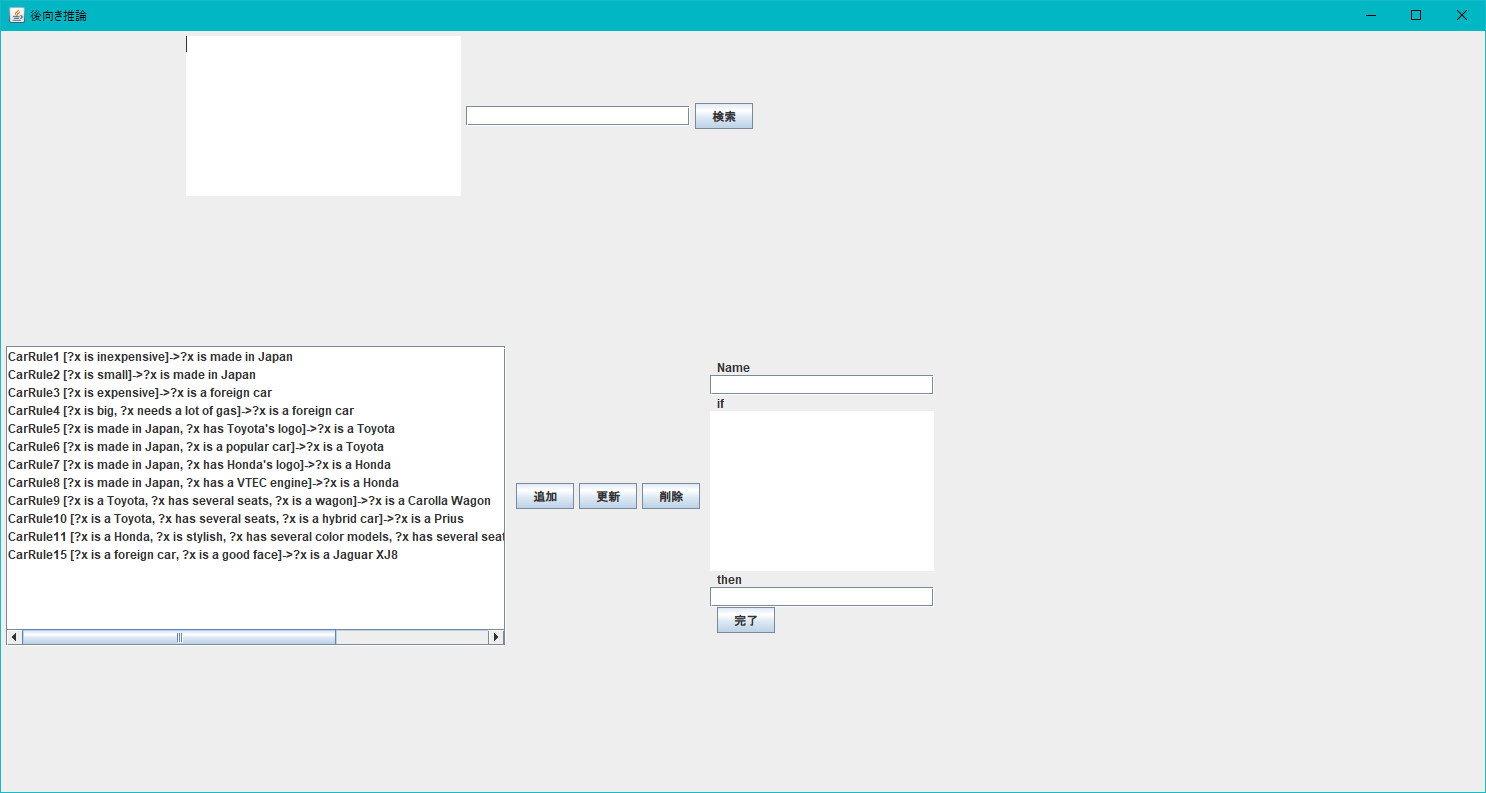
\includegraphics[scale=0.35]{images/gui3.png}
	\end{center}
  	\caption{BwdChainGUI初期状態}
\end{figure}
\clearpage

BwdChainGUIを実行したところ,下図のような画面が得られる.

\begin{figure}[!hbt]
  	\begin{center}
  		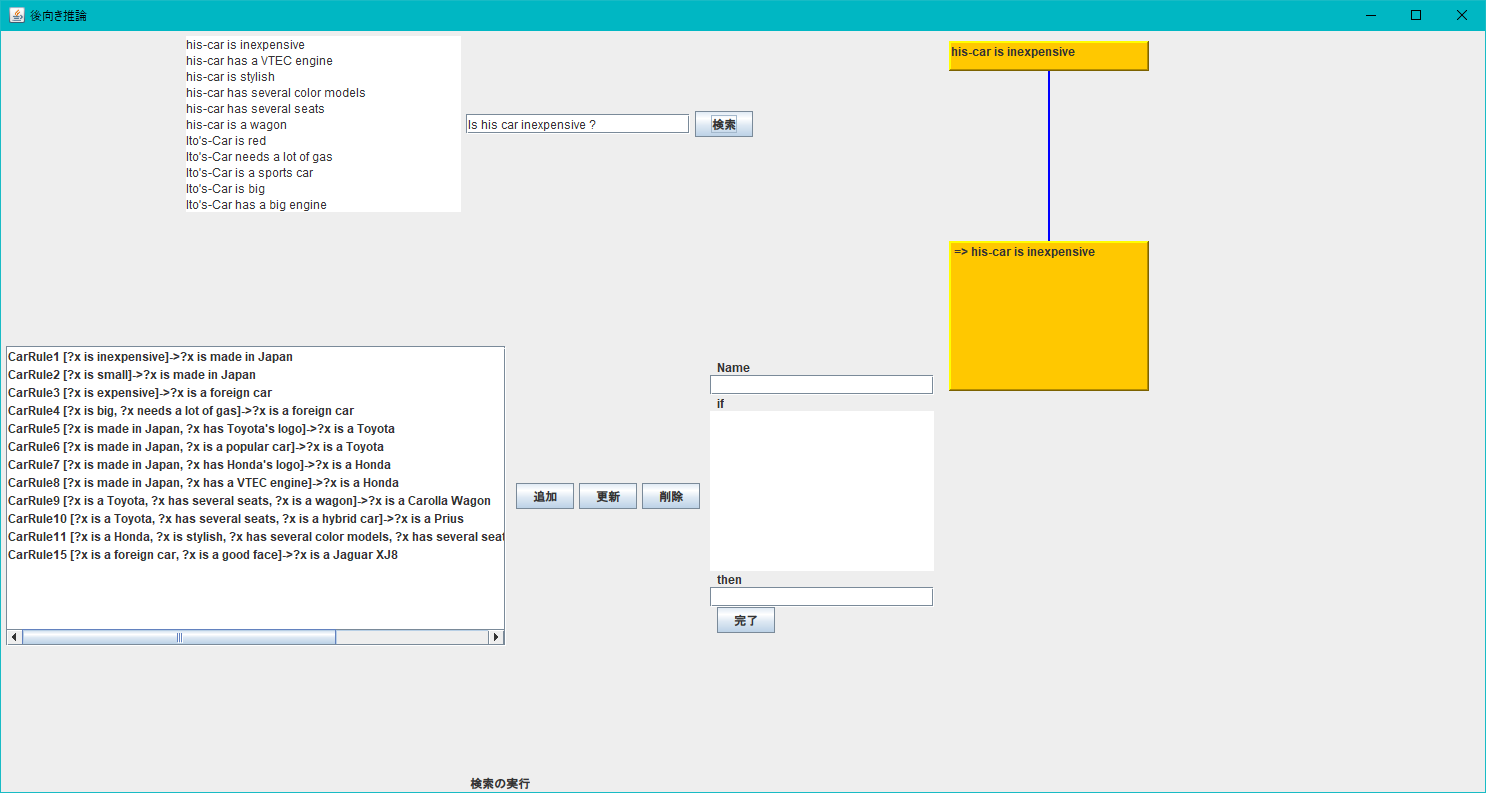
\includegraphics[scale=0.35]{images/gui4.png}
	\end{center}
  	\caption{後向き推論過程を可視化}
\end{figure}
\clearpage


\subsection{考察}
GUIから見た動作としては,前向き推論も後向き推論も似たようなものだと考えられたため,今回の課題ではクラスの抽象化をテーマにして取り組んでみた.初めはChainGUIやChainTableといった抽象クラスにおける前向き・後向きで共通となるであろうメソッドの抽出も出来ていたが,いざPresenterと組み合わせて動作させようとなったときに,Presenter側は抽象化のことを考えていなかったため,後でPresenterの抽象化も試みてはみたが,メソッド名や引数・戻り値の微妙な違いの修正が大変だったため,妥協することとなった.

この経験から,ある程度出来上がってきたものを後で抽象化することは難しく,上手に抽象化するには設計段階でどの部分を抽象化するかを考えてから実装に移る必要があると分かった.以後の課題では,それを考慮して抽象化を活用してゆきたいと思う. \\

今回の課題は今までと取り組み方が異なり,一つ機能を完成させたら次の機能に取り掛かるというアプローチではなく,全体的に未完成なまま作り上げてくというようなアプローチになってしまった.Presenterとのデータの受け渡しが必要だったからやむを得ずということもあったが,今回のアプローチは進捗管理やテスト動作のしづらさから見てもあまり良くなかったと考えられる.

1つの未完成のまま次の機能に取り掛かるにしても,最低限動作するラインまでは次の機能に移ってはいけないと考えられる.そのために,Presenter担当者にも一つの機能の動作の担保を優先して実装してもらうような連携を取り合う必要があったと反省している.

\section{発展課題4-4}
\begin{screen}
上記4-3で実装したGUIを発展させ,質問応答だけでなく,ルールの編集(追加,削除,変更)などについてもGUIで行えるようにせよ.
\end{screen}
私の担当箇所は,発展課題4-4におけるルールの編集機能の,Swingによる実装である.

\subsection{手法}
ルールの編集機能を実装するにあたり,以下のような方針を立てた.
\begin{enumerate}
\item ルールの一覧表示と編集のためのメニューパネルを作る.
\item 追加・更新のためのパネルを作る.
\end{enumerate}

1.に関して,JListクラスを用いてルールの一覧表示を行うことで,ユーザが更新・削除したいルールの選択を視覚的に行えるような仕様とした.

2.に関して,追加・更新のための専用のパネルを用意することで,直感的な編集操作を行えるような仕様とした.

\subsection{実装}
実装に関連するプログラムは,必須課題4-3と同様である.

\subsubsection{ルールの一覧表示と編集のためのメニューパネルを作る}
ルールの表示や編集については,前向き推論においても後向き推論においても共通の処理であるため,FwdChainGUI,BwdChainGUIの抽象クラスであるChainGUIを活用して,実装を行った.

まず,ChainGUIに内部クラスとしてMenuPanelを実装した.MenuPanelでは,JTextFIeldやJTextAreaから入力を受け取り,反映するための各ボタンを実装した.また,JListを用いたルール一覧の表示や,後述するRuleEditorの管理等を行っている.

MenuPanelにおけるボタンが押されたときの動作を表すメソッドactionPerformedをソースコード
\ref{menudone}
に示す.

\begin{lstlisting}[caption=RuleEditorクラスのメソッドactionPerformed, label=menudone]
        @Override
        public void actionPerformed(ActionEvent e) {
            String cmd = e.getActionCommand();

            if (cmd.equals("検索")) {
                ArrayList<String> astList = new ArrayList<>(Arrays.asList(wmTA.getText().split("\n")));
                // ArrayList<String> schAst = new ArrayList<>(Arrays.asList(schTA.getText().split("\n")));  //  複数の質問文のとき?
                ArrayList<String> schAst = new ArrayList<>();
                schAst.add(schTF.getText());

                ctable.schStep(astList, schAst);
            } else {
                if (cmd.equals("追加")) {
                    re.addRule();
                }else if (cmd.equals("更新")) {
                    if (!rulePnl.isSelectionEmpty()) {
                        int index = rulePnl.getSelectedIndex();
                        Rule val = (Rule) rulePnl.getSelectedValue();
                        re.udRule(val);
                    } else {
                        System.out.println("更新失敗(未選択のため)");
                    }
                } else if (cmd.equals("削除")) {
                    if (!rulePnl.isSelectionEmpty()) {
                        int index = rulePnl.getSelectedIndex();
                        Rule val = (Rule) rulePnl.getSelectedValue();
                        ctable.rmRule(val);
                    } else {
                        System.out.println("削除失敗(未選択のため)");
                    }
                }
            }
            status.setText(cmd + "の実行");
        }
\end{lstlisting}

statusラベルのsetTextが最後に呼び出されることによって,RuleEditorのメソッド呼び出しより後に,このactionPerformedメソッドが終了するため,RuleEditorにおけるルール一覧への反映を瞬時に行えるようになっている.

\subsubsection{追加・更新のためのパネルを作る}
MenuPanelの内部クラスとしてRuleEditorを実装した.

Ruleはname部,if部とthen部のそれぞれについて編集を可能とする必要があり,RuleEditorではRuleの追加と編集におけるそれらの包括的な処理が行われるような仕様とした.各フィールドが入力され,完了ボタンが押されたときに,RuleBaseSystemに反映を依頼するメソッドactionPerformedは以下のようになる.

\begin{lstlisting}[caption=RuleEditorクラスのメソッドactionPerformed, label=ruledone]
            @Override
            public void actionPerformed(ActionEvent e) {
                String nameText = nameTF.getText();
                ArrayList<String> ifList = new ArrayList<>(Arrays.asList(ifTA.getText().split("\n")));
                String thenText = thenTF.getText();
    
                if(rule == null) {
                    ctable.addRule(nameText, ifList, thenText);
                } else {
                    ctable.udRule(new Rule(nameText, ifList, thenText));
                }
                udRuleMod();
            }
\end{lstlisting}

ctableはChainTable型のメソッドであり,前向き・後向きそれぞれのChainTableからPresenterを呼び出して反映が行われることが分かる.

また,udRuleModメソッドは以下のようになる.

\begin{lstlisting}[caption=MenuPanelクラスのメソッドudRuleMod, label=udmod]
        void udRuleMod() {
            ruleList = ctable.getRules();
            ruleMod.clear();
            for (Rule r : ruleList) {
                ruleMod.addElement(r);
            }
        }
\end{lstlisting}

これにより,GUI上でのルール一覧の表示の更新が行われている.

\clearpage

\subsection{実行例}
FwdChainGUIを実行したところ,以下のような画面が得られる.なお,BwdChainGUIでも同様の動作をする.

\begin{figure}[!hbt]
  	\begin{center}
  		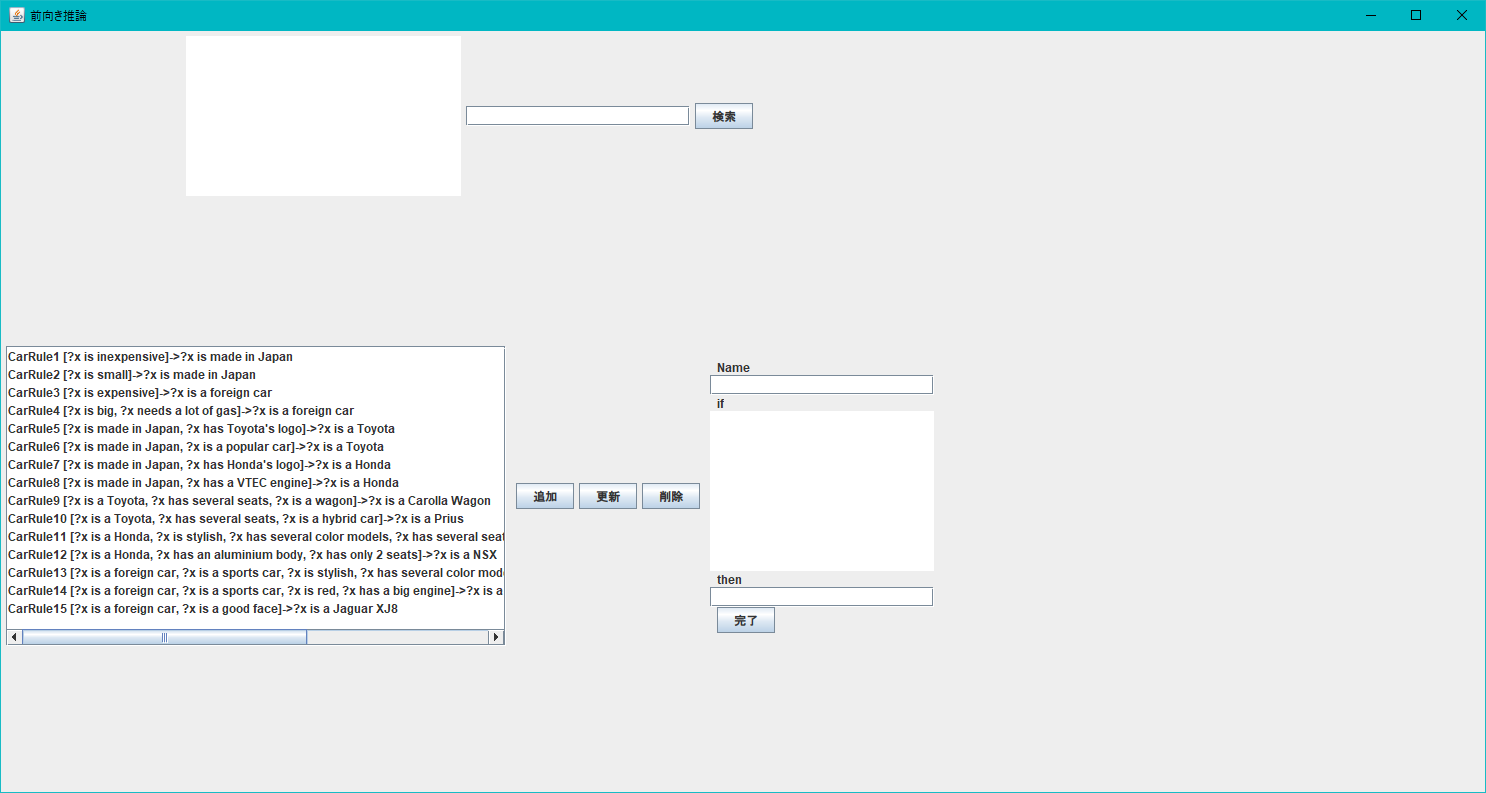
\includegraphics[scale=0.35]{images/gui1.png}
	\end{center}
  	\caption{初期状態}
\end{figure}
\clearpage

Rule5を選択し,削除ボタンを押したところ以下のような画面が得られる.

\begin{figure}[!hbt]
  	\begin{center}
  		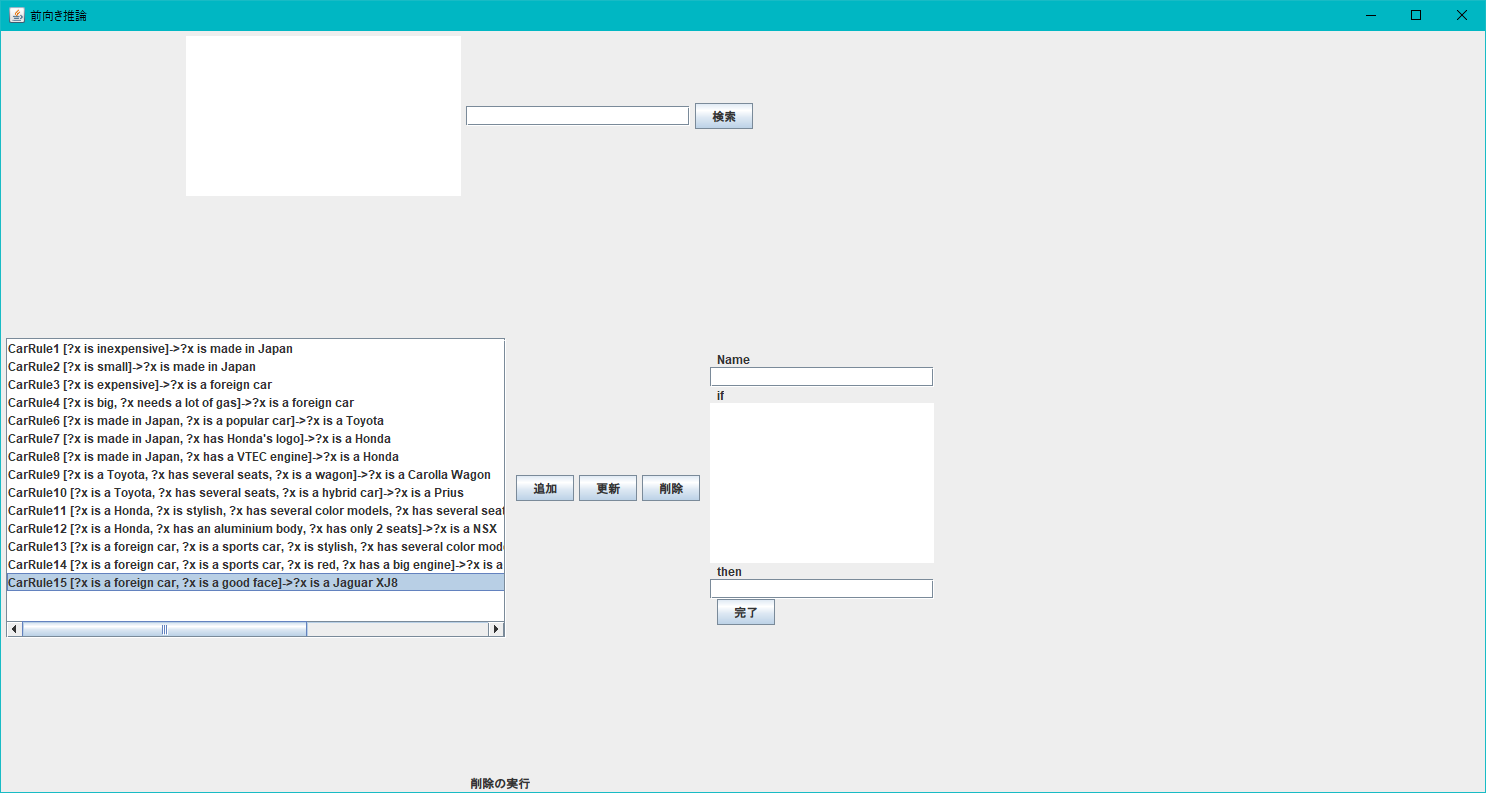
\includegraphics[scale=0.35]{images/gui5.png}
	\end{center}
  	\caption{削除の実行}
\end{figure}
\clearpage

追加ボタンを押し,テキストを入力後,完了ボタンを押したところ以下のような画面が得られる.

\begin{figure}[!hbt]
  	\begin{center}
  		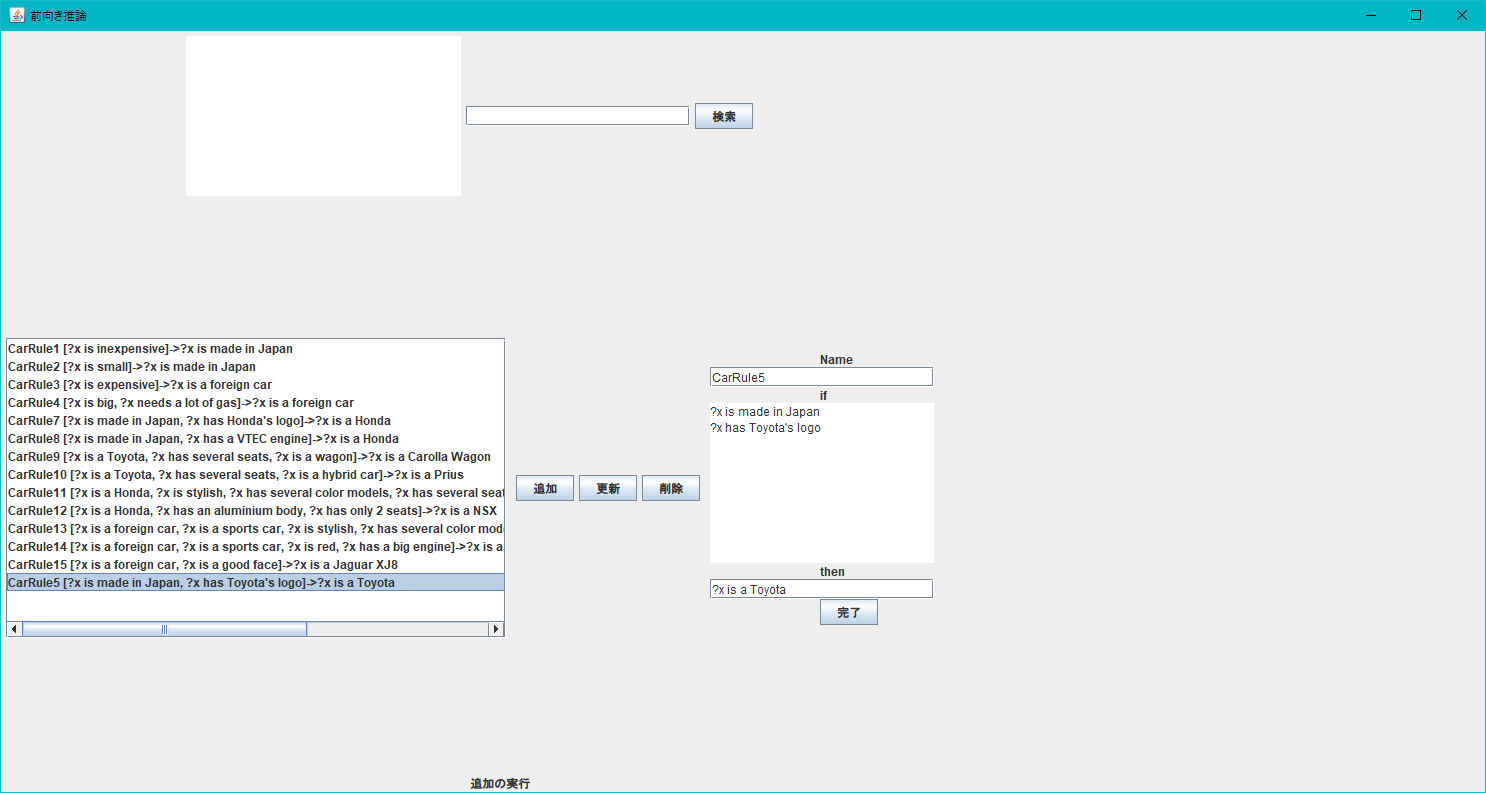
\includegraphics[scale=0.35]{images/gui6.png}
	\end{center}
  	\caption{追加の実行}
\end{figure}
\clearpage

Rule3を選択して更新ボタンを押し,ifのテキストに''?x is big''を加え,完了ボタンを押したところ以下のような画面が得られる.

\begin{figure}[!hbt]
  	\begin{center}
  		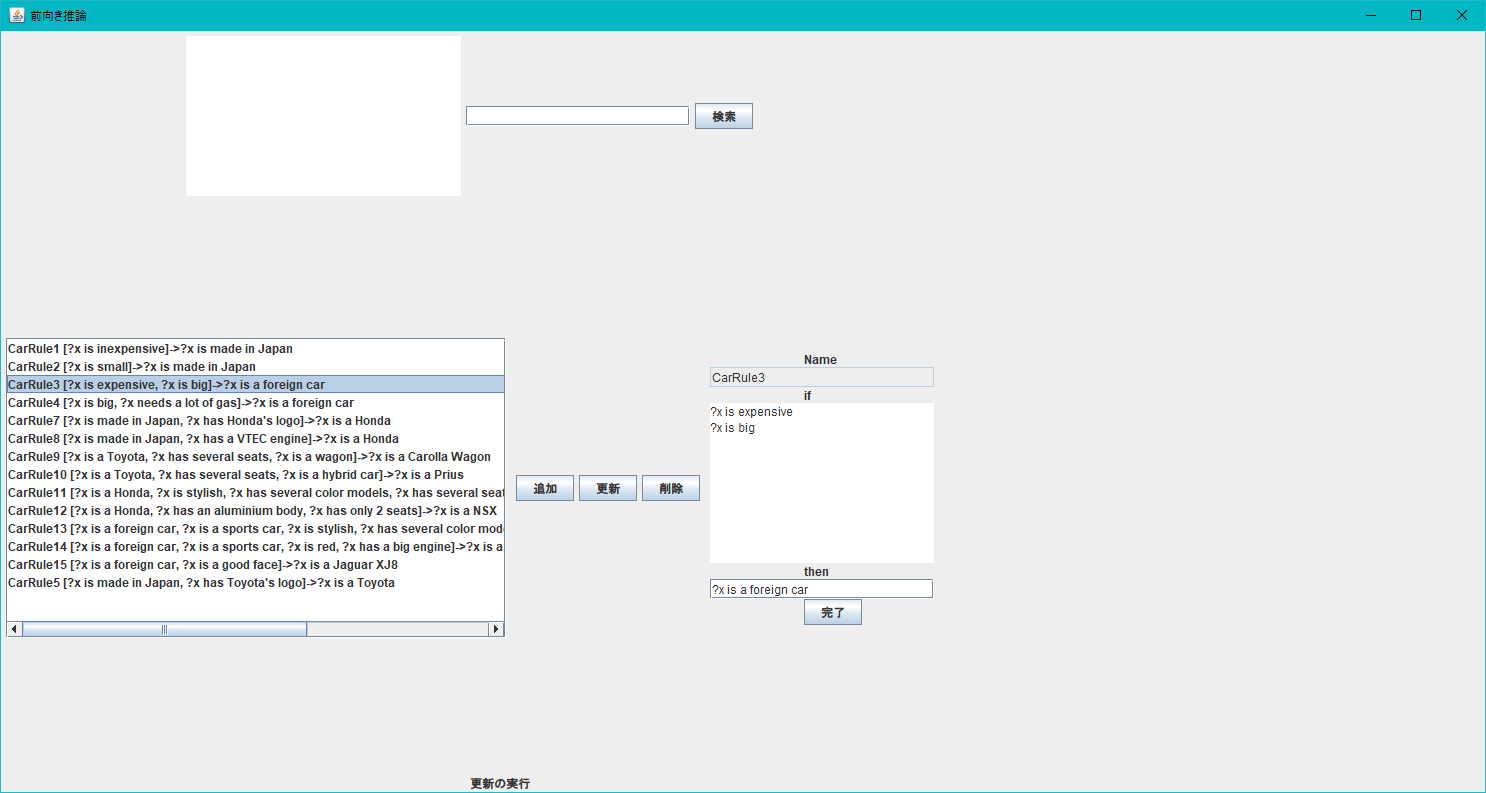
\includegraphics[scale=0.35]{images/gui7.png}
	\end{center}
  	\caption{更新の実行}
\end{figure}
\clearpage

\subsection{考察}
前回までの課題でJListやJButtonを組み合わせた追加・削除は経験しているため,実装はあまり大変ではなかった.

しかし,レイアウトの設定が中々上手にできず,意図とは異なった挙動も所々見られた.例えば,MemuPanelでgetContentPane().addメソッドを利用すると,MenuPanelのインスタンスを生成した元のフレームにおいてそれが反映されてしまうことや,同じくMenuPanelにおいて,BoxLayoutを用いてsetLayoutを行うと,エラーが吐かれてしまうことなどである.

これらの問題はいずれも,LayoutとContainerの違いを正しく理解できていなかったためだと考えられる.おそらくペインを用いた配置については,JPanelではなくJFrameからしか使えないためだと考えられる.やはりSwingにおいても基礎から段階的に学んでいかないと,こういった場面でものの違いが分からずに躓くことが多くなると感じた.

また,イベントモデルについてもあまり理解せずに使っている節がある.例えばルールの更新をしたあとのudRuleModメソッド呼び出しが,ボタンを連打しないと実行されないように見えたりする,という問題が挙げられる.これは実装でも述べたように,statusラベルのsetTextメソッドをudRuleMod後に実行するような仕様とすることで解決したが,これはSwing特有の問題ではなく,まさにマルチスレッド処理における問題であったことにそこで初めて気づいた.イベントモデルのようなメソッドをただ便利だからと使うだけでなく,裏でどんな処理がなされているかを考えることが,問題解決の一つの手段となることを気づいたと同時に,やはりイベントモデルについても基礎から学んでおかないと,解決できてもその場限りのものとなり,自分の中で応用できないものとなりうることに気づいた.

\section{感想}
今回の課題では前回の反省も活かして,班員との仕様の打ち合わせは早い段階から行っていたが,前回よりも実装は大変なものとなった.これはRuleBaseSystemの構造や挙動が前回の課題と比較しても複雑であるため,そこに外部からデータを取り込んだり,内部からデータを取り出すのは大変であったからだと考えられるが,その他にも班員との意識のすれ違いがあったことが大きな要因として挙げられると考えられる.

例えば,GUIの実装側からすると,推論過程を線で繋げて表示するために,内部の挙動的にどのアサーションがどこからきて,どこに繋がってゆくかを知りたいのに,Presenterからは断片的なリストが渡されたりすることや,Presenterから渡される型が独自のものであり,更にはそれもRuleBaseSystem内で実装されているため,Presenterから受け取ったデータのフィールドやメソッドを調べるためにわざわざRuleBaseSystem.javaまで調べないといけなかったりすることが挙げられる.

これらはGUI側としての要求定義が甘かったことも考えられるが,班員のPresenter担当者がGUI未経験であることが要因の一つとして挙げられる.今回の課題で,GUI担当者が本当に欲しいものはGUIを作った経験がある人しか分からないということを痛感したため,次回の課題ではGUIの制作を他の班員に任せ,私がPresenterを担当することで,GUI実装の円滑なサポートと,Presenter担当側から見た,苦悩やGUI担当者から欲しい情報等を学びたいと思った.

また,今回GUIを実装していてRuleBaseSystem.javaをしばし調べ,内部の挙動を知る必要があったが,GUI製作者からすると本当に必要なのはデータの受け渡しだけであるため,次回の課題で実装するPresenterでは,実装するメソッドやクラスの説明も充分にできるよう意識したい.

% 参考文献
\begin{thebibliography}{99}
TATSUO IKURA: 『Swingを使ってみよう - Java GUIプログラミング』 https://www.javadrive.jp/tutorial/ (2019/11/18アクセス) \\
\end{thebibliography}

\end{document}
